\chapter{Applicazioni}

\section{Perturbazioni Stazionarie}

Trattiamo ora il caso delle perturbazioni stazionarie, ovvero quelle in cui l'operatore non dipende esplicitamente dal tempo.
L'Hamiltoniana del sistema è data da:
\begin{equation}
    H = H_0 + W = H_0 + \lambda \hat{W} \qquad \text{con } \lambda \ll 1
\end{equation}
dove $H_0$ è l'\textit{Hamiltoniano imperturbato}, di cui sappiamo risolvere l'equazione agli autovalori e trovare gli autovettori, mentre $W$ rappresenta la perturbazione controllata dal parametro reale $\lambda$.

Lo spettro di $H_0$ è assunto discreto e non degenere (ogni autovalore corrisponde a un singolo autovettore a meno di normalizzazione):
\[
    \sigma(H_0) = \left\{ E_1^0 < E_2^0 < E_3^0 < \dots \right\}
\]
Gli autostati $\{ \ket{E_a^0} \}$ formano una base ortonormale di autovettori, per cui vale $\braket{E_a^0}{E_b^0} = \delta_{ab}$.

Analizziamo il sistema al variare del parametro $\lambda$:
\begin{itemize}
    \item Per $\lambda = 0$ conosciamo tutto del sistema (caso imperturbato).
    \item Per $\lambda$ piccoli (in un intorno di zero), supponiamo che le grandezze cambino con continuità.
\end{itemize}
Gli autovalori $E_a^\lambda$ cambiano al variare di $\lambda$. Sebbene possa verificarsi il fenomeno del \textit{level crossing} (incrocio dei livelli), noi ci limitiamo a piccole variazioni dove l'ordine dei livelli tende a preservarsi e rimaniamo "prima" che varino troppo.

Vogliamo risolvere l'equazione agli autovalori per l'Hamiltoniana completa:
\begin{equation}
    \label{eq: pertubazioni}
    (H(\lambda) - E_a^\lambda) \ket{E_a^\lambda} = 0 \quad \iff \quad H\ket{E_a^\lambda} = E_a^\lambda \ket{E_a^\lambda}
\end{equation}
Sia gli autovalori che gli autovettori dipendono da $\lambda$. Se $\lambda$ è sufficientemente piccolo, i corrispondenti autovalori rimangono non degeneri (ad esempio, se $E_1^0$ è il livello fondamentale non degenere, per $\lambda$ piccoli rimarrà il più basso e l'autospazio rimarrà di dimensione 1).
Valgono i limiti per $\lambda \to 0$:
\[
    \ket{E_a^\lambda} \xrightarrow{\lambda \to 0} \ket{E_a^0} \qquad E_a^\lambda \xrightarrow{\lambda \to 0} E_a^0
\]

\begin{figure}[ht]
    \centering
    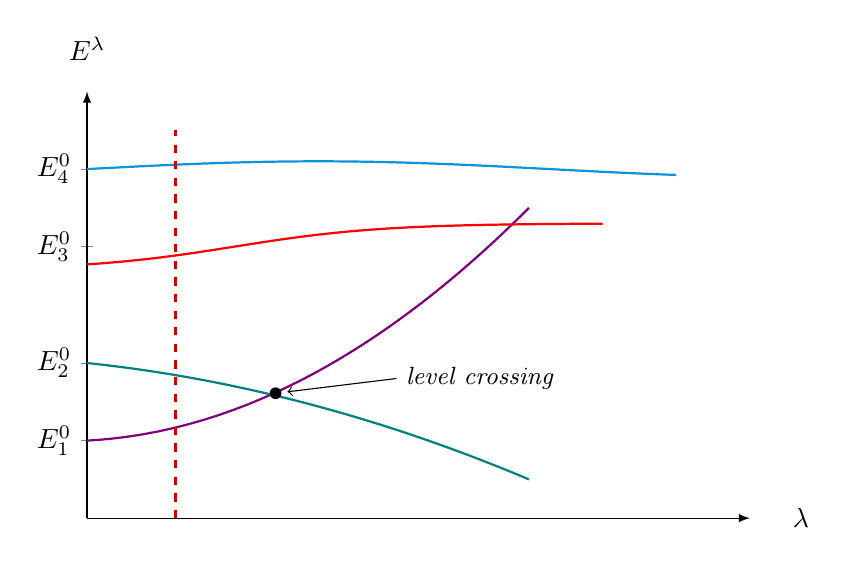
\begin{tikzpicture}
        \begin{axis}[
            axis lines=middle,
            xlabel={$\lambda$},
            ylabel={$E^\lambda$},
            xtick=\empty,
            ytick={1, 2, 3.5, 4.5},
            yticklabels={$E_1^0$, $E_2^0$, $E_3^0$, $E_4^0$},
            ymin=0, ymax=5.5,
            xmin=0, xmax=4.5,
            width=10cm, height=7cm,
            clip=false,
            axis line style={-latex},
            every axis y label/.style={at={(ticklabel* cs:1.05)}, anchor=south},
            every axis x label/.style={at={(ticklabel* cs:1.05)}, anchor=west}
        ]

        % E1 (viola): parte dal basso e sale incrociando
        \addplot[thick, violet, domain=0:3, samples=100, smooth] {1 + 0.1*x + 0.3*x^2};

        % E2 (verde petrolio): parte da sopra e scende incrociando
        \addplot[thick, teal, domain=0:3, samples=100, smooth] {2 - 0.2*x - 0.1*x^2};

        % E3 (rosso): sale
        \addplot[thick, red, domain=0:3.5, samples=100, smooth] {3.5 + 0.3*tanh(x-1)};

        % E4 (ciano): rimane quasi costante
        \addplot[thick, cyan!80!blue, domain=0:4, samples=100, smooth] {4.5 + 0.1*sin(deg(x))};

        % Level crossing
        % Punto di incrocio approssimativo
        \node[circle, fill, inner sep=1.5pt] (crossing) at (axis cs:1.28, 1.61) {};
        
        % Etichetta spostata più a destra per evitare sovrapposizioni
        % (tra la curva viola che sale e la verde che scende)
        \node[right, align=left] (label) at (axis cs:2.1, 1.8) {\small \textit{level crossing}};
        
        % Freccia che punta al crossing
        \draw[->, shorten >= 2pt] (label.west) -- (crossing);

        % Linee tratteggiate verticali (opzionali per stile)
        \draw[dashed, red!80!black, thick] (axis cs:0.6, 0) -- (axis cs:0.6, 5);

        \end{axis}
    \end{tikzpicture}
    \caption{Livelli energetici in funzione del parametro perturbativo $\lambda$.}
    \label{fig:level_crossing}
\end{figure}

Fissiamo un livello \( a \) tale per cui \( \ket{\lambda} \equiv \ket{E_a^\lambda} \) e \( E^\lambda \equiv E_a^\lambda \).
Consideriamo lo sviluppo in serie di Taylor per studiare come cambiano autovalori e autovettori, abbiamo:
\begin{equation}
    E^\lambda = \mathcal{E}_0 + \mathcal{E}_1 \lambda + \mathcal{E}_2 \lambda^2 + \dots + \mathcal{E}_n \lambda^n + O(\lambda^{n+1})
\end{equation}
dove identifichiamo il termine di ordine zero con il livello imperturbato \( \mathcal{E}_0 = E_a^0 \), mentre \( \mathcal{E}_1 \) rappresenta la correzione al primo ordine e così via.

Analogamente, fissiamo anche il vettore di stato:
\begin{equation}
    \ket{E^\lambda} = \ket{\lambda} = \ket{0} + \lambda \ket{1} + \lambda^2 \ket{2} + \dots + \lambda^n \ket{n} + O(\lambda^{n+1})
\end{equation}
dove \( \ket{0} = \ket{E_a^0} \) è lo stato imperturbato noto e gli altri termini \( \ket{1}, \ket{2}, \dots \) sono le correzioni incognite.\\
In questo modo otteniamo delle soluzioni approssimate di autovalori e autovettori trascurando i termini di ordine \( \lambda^{n+1} \).

\begin{attention}
    Esiste un problema di ambiguità nella definizione di \( \ket{\lambda} \): possiamo sempre riscalare il vettore.
    \[
        \ket{\lambda} \longrightarrow c(\lambda) \ket{\lambda}
    \]
    Poiché \( \forall \lambda \) posso riscalare il vettore in maniera diversa (mettendo \( c \in \mathbb{C} \) in funzione di \( \lambda \)), è necessario imporre delle condizioni per rimuovere questa ambiguità:
    \begin{itemize}
        \item Fissiamo lo stato imperturbato: \( \ket{E_a^0} \equiv \ket{0} \) con \( \braket{0}{0}=1 \).
        \item Normalizzazione: \( \braket{\lambda}{\lambda} = 1 \quad \forall \lambda \in \mathbb{R} \).
        \item Fase: impongo \( \braket{0}{\lambda} \in \mathbb{R} \implies \braket{0}{n} = \braket{n}{0} \quad \forall n \).
    \end{itemize}

    Sviluppiamo la condizione di normalizzazione al primo ordine:
    \begin{align*}
        1 = \braket{\lambda}{\lambda} &= \big( \bra{0} + \lambda \bra{1} + \dots \big) \big( \ket{0} + \lambda \ket{1} + \dots \big) \\
        &= \underbrace{\braket{0}{0}}_{1} + \lambda \underbrace{\big( \braket{1}{0} + \braket{0}{1} \big)}_{2\braket{0}{1}} + O(\lambda^2)
    \end{align*}
    Da cui si ricava la condizione: \(\braket{0}{1} = 0\) .\\
    Se espando fino a \(\lambda^3\), avrò la condizione \(\braket{2}{0}= \braket{0}{2}= - \frac{1}{2}\braket{1}{1}\) e il vettore rimane unico.
\end{attention}

La nostra equazione agli autovalori (\ref{eq: pertubazioni}) diventa:
\begin{equation}
    \left(H_0+ \lambda\hat{W}- \sum_{n=0}^{\infty}\epsilon_n\lambda^n\right)\sum_{k=0}^{\infty}\lambda^k\ket{k}=0 \qquad \forall \,\lambda
\end{equation}

Otteniamo così le equazioni per le correzioni \(\epsilon_n\) fermandoci all'ordine che ci interessa:
\begin{align*}
    \lambda^0 &: \quad (H_0 - \varepsilon_0) \ket{0} = 0 \\
    \lambda^1 &: \quad (H_0 - \varepsilon_0) \ket{1} + (\hat{W} - \varepsilon_1) \ket{0} = 0 \\
    \lambda^2 &: \quad (H_0 - \varepsilon_0) \ket{2} + (\hat{W} - \varepsilon_1) \ket{1} - \varepsilon_2 \ket{0} = 0 \\
    &\vdots \\
    \lambda^q &: \quad (H_0 - \varepsilon_0) \ket{q} + (\hat{W} - \varepsilon_1) \ket{q-1} - \varepsilon_2 \ket{q-2} - \dots - \varepsilon_q \ket{0} = 0 \\
    &\vdots
\end{align*}

% 27 Lezione del 01/12/2025


\begin{remark}
    \lezione{27}{01/12/2025}
    Non è necessario richiedere la convergenza della serie perturbativa completa. 
    È sufficiente che la funzione sia abbastanza regolare da ammettere uno sviluppo fino all'ordine finito desiderato. 
    In tal caso, il teorema di Lagrange garantisce che il resto (l'errore commesso troncando la serie) sia infinitesimo per \(\lambda \to 0\), 
    anche qualora la serie di Taylor completa non fosse convergente (comportamento asintotico).
\end{remark}

Per l'ordine \(\lambda^0\) identifichiamo l'energia e lo stato imperturbati:
\[
    \varepsilon_0 = E_a^0 \qquad \ket{0} = \ket{E_a^0}
\]

Per l'ordine \(\lambda^1\), proiettando l'equazione correttiva sul bra imperturbato \(\bra{E_a^0}\), otteniamo:
\[
    \underbrace{\mel{E_a^0}{H_0 - \varepsilon_0}{1}}_{=0} + \mel{E_a^0}{\hat{W} - \varepsilon_1}{0} = 0
\]
Il primo termine si annulla poiché \(\bra{E_a^0}(H_0 - E_a^0) = 0\). Sviluppando il secondo termine e sapendo che \(\ket{0}=\ket{E_a^0}\):
\[
    \mel{E_a^0}{\hat{W}}{E_a^0} = \varepsilon_1 \underbrace{\braket{0}{0}}_{=1}
\]
Otteniamo dunque la correzione al primo ordine per l'energia \(\varepsilon_1 = \mel{E_a^0}{\hat{W}}{E_a^0}\).
L'energia totale dello stato perturbato risulta quindi:
\[
    E_a^\lambda = E_a^0 + \mel{E_a^0}{\lambda \hat{W}}{E_a^0} + O(\lambda^2)
\]

Per ottenere la correzione allo stato \(\ket{1}\), proiettiamo l'equazione perturbativa sul bra \(\bra{E_b^0}\) con \(b \neq a\):
\[
    \mel{E_b^0}{H_0 - \varepsilon_0}{1} + \mel{E_b^0}{\hat{W} - \varepsilon_1}{0} = 0
\]
\[
    (E_b^0 - E_a^0) \braket{E_b^0}{1} + \mel{E_b^0}{\hat{W}}{E_a^0} -\epsilon_1\braket{E_b^0}{E_a^0} = 0
\]
Possiamo ora ricavare i coefficienti dello sviluppo di \(\ket{1}\) lungo la base imperturbata (per \(b \neq a\)):
\begin{equation}
    \braket{E_b^0}{1} = \frac{\mel{E_b^0}{\hat{W}}{E_a^0}}{E_a^0 - E_b^0}
\end{equation}
Lo stato corretto al primo ordine si scrive espandendo sulla base completa. Precedentemente abbiamo supposto \(\braket{E_a^0}{1} = 0\), dunque:
\[
    \ket{1} = \sum_{b} \ket{E_b^0}\braket{E_b^0}{1} = \underbrace{\braket{E_a^0}{1}}_{0} \ket{E_a^0} + \sum_{b \neq a} \frac{\mel{E_b^0}{\hat{W}}{E_a^0}}{E_a^0 - E_b^0} \ket{E_b^0}
\]
Dunque, lo stato totale fino all'ordine \(\lambda\) è:
\begin{equation}
    \ket{E_a^\lambda} = \ket{E_a^0} + \lambda \sum_{b \neq a} \frac{\mel{E_b^0}{\hat{W}}{E_a^0}}{E_a^0 - E_b^0} \ket{E_b^0} + O(\lambda^2)
\end{equation}


Per ottenere \(\varepsilon_2\), consideriamo l'equazione perturbativa di ordine \(\lambda^2\) proiettata su \(\bra{E_a^0}\):
\[
    \mel{E_a^0}{H_0 - \varepsilon_0}{2} + \mel{E_a^0}{\hat{W} - \varepsilon_1}{1} - \varepsilon_2 \braket{E_a^0}{0} = 0
\]
Il primo termine è nullo (\(\bra{E_a^0}(H_0 - E_a^0) = 0\)). Sapendo che \(\ket{0} = \ket{E_a^0}\), abbiamo \(\braket{E_a^0}{0} = 1\). Inoltre, abbiamo imposto \(\braket{E_a^0}{1} = 0\), quindi il termine con \(\varepsilon_1\) si annulla. Rimane:
\[
    \mel{E_a^0}{\hat{W}}{1} = \varepsilon_2
\]
Sostituendo l'espressione di \(\ket{1}\) trovata in precedenza:
\begin{equation}
    \varepsilon_2 = \sum_{b \neq a} \mel{E_a^0}{\hat{W}}{E_b^0} \braket{E_b^0}{1} 
        = \sum_{b \neq a} \frac{\mel{E_a^0}{\hat{W}}{E_b^0} \mel{E_b^0}{\hat{W}}{E_a^0}}{E_a^0 - E_b^0}
        = \sum_{b \neq a} \frac{\abs{\mel{E_b^0}{\hat{W}}{E_a^0}}^2}{E_a^0 - E_b^0}
\end{equation}
L'energia totale corretta fino all'ordine \(\lambda^2\) è:
\begin{equation}
    E_a^\lambda = E_a^0 + \lambda \mel{E_a^0}{\hat{W}}{E_a^0} + \lambda^2 \sum_{b \neq a} \frac{\abs{\mel{E_b^0}{\hat{W}}{E_a^0}}^2}{E_a^0 - E_b^0} + O(\lambda^3)
\end{equation}

\subsection{Correzione armonica oscillatore armonico}

Consideriamo l'hamiltoniana dell'oscillatore armonico con una perturbazione cubica:
\[
    H = H_0 + W \qquad \text{con} \quad H_0 = \frac{P^2}{2m} + \frac{1}{2}m\omega^2 X^2 = \frac{\hbar\omega}{2}\left( \hat{P}^2 + \hat{X}^2 \right)
\]
La perturbazione è definita come:
\begin{equation}
    W = \lambda \hat{W} = \lambda \hbar \omega \hat{X}^3 \qquad \text{con } \abs{\lambda} \ll 1
\end{equation}
Ricordiamo le proprietà degli autostati \(\ket{E_n^0}\equiv\ket{n}\) dell'hamiltoniana imperturbata:
\[
    H_0 \ket{n} = E_n^0 \ket{n} \qquad E_n^0 = \hbar\omega\left(n + \frac{1}{2}\right)
\]
Esprimiamo l'operatore posizione \(\hat{X}\) tramite gli operatori di scaletta:
\[
    \hat{X} = \frac{a + a^\dagger}{\sqrt{2}} \qquad N = a^\dagger a \qquad [a, a^\dagger] = 1 \implies a a^\dagger = N + 1
\]
L'azione degli operatori sugli stati è data da:
\[
    a^\dagger \ket{n} = \sqrt{n+1}\ket{n+1} \qquad a \ket{n} = \sqrt{n}\ket{n-1}
\]

Calcoliamo ora l'operatore \(\hat{W}\) espandendo il cubo della posizione:
\[
    \hat{W} = \hbar\omega \hat{X}^3 = \frac{\hbar\omega}{2\sqrt{2}} (a + a^\dagger)^3
\]
Sviluppiamo il cubo mantenendo l'ordine degli operatori e raggruppiamo i termini utilizzando le identità dell'operatore numero \(N\):
\begin{align*}
    (a + a^\dagger)^3 &= a^3 + (a^\dagger)^3 \\
    &\quad + \underbrace{a^\dagger a a}_{Na} + \underbrace{a a^\dagger a}_{(N+1)a} + \underbrace{a a a^\dagger}_{(N+2)a} \\
    &\quad + \underbrace{a^\dagger a^\dagger a}_{(N-1)a^\dagger} + \underbrace{a^\dagger a a^\dagger}_{N a^\dagger} + \underbrace{a a^\dagger a^\dagger}_{(N+1)a^\dagger}
\end{align*}
Sommando i coefficienti per \(a\) e \(a^\dagger\):
\begin{itemize}
    \item Termini in \(a\): \(N + (N+1) + (N+2) = 3N + 3 = 3(N+1)\)
    \item Termini in \(a^\dagger\): \((N-1) + N + (N+1) = 3N\)
\end{itemize}
Otteniamo infine l'espressione in forma normale per la perturbazione:
\begin{equation}
    \hat{W} = \frac{\hbar\omega}{2\sqrt{2}} \left[ a^3 + (a^\dagger)^3 + 3(N+1)a + 3N a^\dagger \right]
\end{equation}

Applichiamlo allo stato fondamentale:
\[
\begin{split}
    \hat{W}\ket{E_n^0} = \frac{\hbar \omega}{2\sqrt{2}} \bigg( &\sqrt{n(n-1)(n-2)} \ket{E_{n-3}^0} + \sqrt{(n+1)(n+2)(n+3)} \ket{E_{n+3}^0} \\
    &+ 3 \sqrt{n} \, n \ket{E_{n-1}^0} + 3 \sqrt{n+1} \, (n+1) \ket{E_{n+1}^0} \bigg)
\end{split}
\]
Otteniamo così i valori della correzione dell'energia:
\[
    \varepsilon_1 = \mel{E_n^0}{\hat{W}}{E_n^0} = 0 
\]
\[
    \varepsilon_2 = \sum_{k \neq 0} \frac{\abs{\mel{E_{n+k}^0}{\hat{W}}{E_n^0}}^2}{E_n^0 - E_{n+k}^0}=
\]
\[
    = \frac{\hbar^2 \omega^2}{8} \frac{1}{\hbar \omega} \left( \frac{n(n-1)(n-2)}{3} + \frac{(n+1)(n+2)(n+3)}{-3} + \frac{9n^3}{1} + \frac{9(n+1)^3}{-1} \right)=
\]
\[
    = -\frac{\hbar \omega}{8} ( 30 n^2 + 30 n + 11 )
\]
Dunque l'energia vale:
\begin{equation}
    \implies E_n \approx \hbar \omega \left(n + \frac{1}{2}\right) - \lambda^2 \frac{\hbar \omega}{8} ( 30 n^2 + 30 n + 11 ) + O(\lambda^3)
\end{equation}

\subsection{Caso degenere}
Sia $\mathcal{H}_0$ l'autospazio di $H_0$ relativo all'autovalore $E_a^0 \equiv \varepsilon_0$, con $\dim \mathcal{H}_0 = d$.
Definiamo una base ortonormale di $\mathcal{H}_0$:
\begin{equation}
    \{ \ket{\Phi, r} \}_{r=1,\dots,d} \quad \text{t.c.} \quad \braket{\Phi,r}{\Phi,s} = \delta_{rs}
\end{equation}
L'equazione agli autovalori per l'hamiltoniana perturbata è:
\begin{equation}
    H(\lambda)\ket{E^k(\lambda)} = E^k(\lambda)\ket{E^k(\lambda)} \quad k=1,\dots,d
\end{equation}
Le diverse energie $E^k(\lambda)$ potrebbero "diramarsi" partendo dal livello degenere imperturbato.
Vale il limite $\lim_{\lambda \to 0} E^k(\lambda) = E(0) = \varepsilon_0$.
Possiamo scrivere le espansioni in serie di potenze di $\lambda$:
\[
\begin{aligned}
    E^k(\lambda) &= \varepsilon_0 + \lambda \varepsilon_1^k + \lambda^2 \varepsilon_2^k + \dots \\
    \ket{E^k(\lambda)} &= \ket{0_k} + \lambda \ket{1_k} + \lambda^2 \ket{2_k} + \dots
\end{aligned}
\]
dove $\ket{0_k} = \lim_{\lambda \to 0} \ket{E^k(\lambda)} \in \mathcal{H}_0$.

Inserendo le espansioni nell'equazione di Schrödinger e separando gli ordini, otteniamo per l'ordine generico $\lambda^q$:
\[
    (H_0 - \varepsilon_0)\ket{q_k} + (\hat{W} - \varepsilon_1^k)\ket{(q-1)_k} - \varepsilon_2^k\ket{(q-2)_k} - \dots - \varepsilon_q^k \ket{0_k} = 0
\]

Proiettiamo l'equazione perturbativa al primo ordine su un generico stato della base degenere $\ket{\Phi, r}$:
\[
    \mel{\Phi,r}{H_0 - \varepsilon_0}{1_k} + \mel{\Phi,r}{\hat{W} - \varepsilon_1^k}{0_k} = 0
\]
Poiché $\bra{\Phi,r}(H_0 - \varepsilon_0) = 0$, il primo termine scompare. Otteniamo quindi:
\[
    \mel{\Phi,r}{\hat{W}}{0_k} = \varepsilon_1^k \braket{\Phi,r}{0_k}
\]
Sviluppiamo lo stato di ordine zero $\ket{0_k}$ sulla base di $\mathcal{H}_0$, cioè $\ket{0_k} = \sum_{s=1}^d c_s^k \ket{\Phi,s}$ dove $c_s^k = \braket{\Phi,s}{0_k}$. Inserendo questa espansione otteniamo:
\[
    \sum_{s=1}^d \mel{\Phi,r}{\hat{W}}{\Phi,s} c_s^k = \varepsilon_1^k c_r^k
\]
Definendo la matrice della perturbazione nel sottospazio degenere come $\mathcal{W}_{rs} = \mel{\Phi,r}{\hat{W}}{\Phi,s}$, arriviamo al sistema lineare:
\[
    \begin{pmatrix}
        \mathcal{W}_{11} & \dots & \mathcal{W}_{1d} \\
        \vdots & \ddots & \vdots \\
        \mathcal{W}_{d1} & \dots & \mathcal{W}_{dd}
    \end{pmatrix}
    \begin{pmatrix}
        c_1^k \\ \vdots \\ c_d^k
    \end{pmatrix}
    = \lambda \varepsilon_1^k
    \begin{pmatrix}
        c_1^k \\ \vdots \\ c_d^k
    \end{pmatrix}
\]
È un'equazione agli autovalori per la matrice $\mathcal{W}$.

\begin{itemize}
    \item Gli autovalori $\{\varepsilon_1^1, \dots, \varepsilon_1^d\}$ rappresentano le correzioni energetiche al primo ordine.
    \item Gli autovettori $(c_1^k, \dots, c_d^k)^T$ definiscono gli stati $\ket{0_k}$ (i "buoni" stati di ordine zero) lungo i quali il sistema evolve accendendo la perturbazione.
    \item Se gli autovalori sono tutti distinti (non degeneri), la degenerazione di $E(0)$ è completamente rimossa. Altrimenti, la degenerazione potrebbe essere rimossa a ordini superiori o restare tale.
\end{itemize}

Per semplificare la diagonalizzazione di $\mathcal{W}$, possiamo cercare una base $\{\ket{\Phi,r}\}$ opportuna.
Se esiste un osservabile $A$ tale che:
\[
    [A, H_0] = 0 = [A, \hat{W}]
\]
allora scegliamo $\{\ket{\Phi,r}\}$ come autovettori simultanei di $H_0$ e $A$.
Se $A\ket{\Phi,r} = a_r\ket{\Phi,r}$ e $A\ket{\Phi,s} = a_s\ket{\Phi,s}$ con $a_r \neq a_s$, allora l'elemento di matrice si annulla:
\[
    \mathcal{W}_{rs} = \mel{\Phi,r}{\hat{W}}{\Phi,s} = 0
\]
Questo rende la matrice $\mathcal{W}$ diagonale a blocchi, facilitando il calcolo degli autovalori.

\subsection{Oscillatore armonico 2D}

Consideriamo lo spazio di Hilbert prodotto tensoriale degli spazi 1D:
\[
    \mathcal{H} = L_2(\mathbb{R}, \dd{x}) \otimes L_2(\mathbb{R}, \dd{y}) = L_2(\mathbb{R}^2, \dd{x}\dd{y})
\]

L'Hamiltoniana del sistema è data dalla somma delle Hamiltoniane lungo gli assi:
\[
    H_0 = \frac{P_x^2 + P_y^2}{2m} + \frac{1}{2}m\omega^2(X^2 + Y^2) = H_{0x} + H_{0y}
\]
Utilizzando le variabili adimensionali, possiamo riscriverla come:
\[
    H_0 = \frac{\hbar\omega}{2} \left( \hat{P}_x^2 + \hat{X}^2 + \hat{P}_y^2 + \hat{Y}^2 \right)
\]

Definiamo gli operatori di distruzione per ciascuna coordinata:
\[
    a_x = \frac{\hat{X} + i\hat{P}_x}{\sqrt{2}} \qquad a_y = \frac{\hat{Y} + i\hat{P}_y}{\sqrt{2}}
\]
e i rispettivi operatori numero:
\[
    N_x = a_x^\dagger a_x \qquad N_y = a_y^\dagger a_y
\]

Gli autostati di \( H_0 \) sono il prodotto tensoriale degli autostati 1D:
\[
    \ket{n_x, n_y} \equiv \ket{n_x} \otimes \ket{n_y}
\]
L'equazione agli autovalori risulta:
\[
    H_0 \ket{n_x, n_y} = \hbar\omega(n_x + n_y + 1)\ket{n_x, n_y} \qquad n_x, n_y = 0, 1, 2, \dots
\]

I livelli energetici sono dati da \( E_n^0 = \hbar\omega(n+1) \) ponendo \( n = n_x + n_y \). Analizziamo i primi livelli e la loro degenerazione:
\begin{align*}
    E_0^0 &= \hbar\omega \quad && \ket{0,0} \\
    E_1^0 &= 2\hbar\omega \quad && \ket{1,0}, \ket{0,1} \\
    E_2^0 &= 3\hbar\omega \quad && \ket{2,0}, \ket{1,1}, \ket{0,2} \\
    &\vdots &&
\end{align*}

Consideriamo ora una perturbazione della forma \( W = \lambda \hbar \omega \hat{X}\hat{Y} \). Esprimendola tramite gli operatori di creazione e distruzione:
\begin{equation}
    W = \lambda \hbar \omega \hat{X}\hat{Y} = \frac{\lambda \hbar \omega}{2} (a_x + a_x^\dagger)(a_y + a_y^\dagger)
    = \frac{\lambda \hbar \omega}{2} \left( a_x a_y + a_x^\dagger a_y + a_x a_y^\dagger + a_x^\dagger a_y^\dagger \right)
\end{equation}

Analizziamo le correzioni energetiche al primo ordine, $o(\lambda^1)$, per i primi livelli energetici.

% 28 Lezione del 05/12/2025

\paragraph{Stato fondamentale $E_0^0$}

\lezione{28}{05/12/2025}

Lo stato fondamentale $\ket{0,0}$ è non degenere. La correzione al primo ordine è data dal valor medio della perturbazione sullo stato indeperturbato:
\[
    \Delta E_0^1 = \mel{0,0}{W}{0,0} = 0
\]
Poiché $W$ contiene combinazioni di operatori di creazione e distruzione che, applicati a $\ket{0,0}$, producono stati ortogonali o nulli, il valor medio è zero.

\paragraph{Primo stato eccitato $E_1^0$}
Il livello $E_1^0$ ha degenerazione $g=2$. La base dell'autospazio è data da:
\[
    \left\{ \ket{1,0} \equiv \ket{\phi_1},\; \ket{0,1} \equiv \ket{\phi_2} \right\}
\]
Dobbiamo calcolare la matrice della perturbazione nel sottospazio degenere, definita da $\mathcal{W}_{rs} = \mel{\phi_r}{W}{\phi_s}$.

Calcoliamo gli elementi di matrice. I termini diagonali sono nulli:
\[
    \mel{1,0}{W}{1,0} = 0 \quad \text{e} \quad \mel{0,1}{W}{0,1} = 0
\]
I termini fuori diagonale sono non nulli. Ad esempio:
\[
    \mel{1,0}{W}{0,1} = \frac{\lambda \hbar \omega}{2} \mel{1,0}{a_x^\dagger a_y}{0,1} = \frac{\lambda \hbar \omega}{2} \braket{1,0}{1,0} = \frac{\lambda \hbar \omega}{2}
\]
Similmente $\mel{0,1}{W}{1,0} = \frac{\lambda \hbar \omega}{2}$. La matrice $\mathcal{W}$ risulta:
\[
    \mathcal{W} = \frac{\lambda \hbar \omega}{2} 
    \begin{pmatrix}
        0 & 1 \\
        1 & 0
    \end{pmatrix}
\]

Diagonalizzando $\mathcal{W}$ troviamo gli autovalori (le correzioni all'energia):
\[
    \det(\mathcal{W} - \varepsilon \mathbb{I}) = 0 \implies \varepsilon^2 - \left(\frac{\lambda\hbar\omega}{2}\right)^2 = 0 \implies \Delta E_{1\pm}^1 = \pm \frac{\lambda \hbar \omega}{2}
\]
I corrispondenti autovettori, che costituiscono la "base corretta" per la perturbazione, sono:
\[
    \ket{\pm} = \frac{\ket{0,1} \pm \ket{1,0}}{\sqrt{2}}
\]

In conclusione, l'energia del primo stato eccitato si separa in due livelli distinti (rimozione della degenerazione):
\begin{equation}
    E_1^{\pm}(\lambda) = E_1^0 \pm \frac{\lambda \hbar \omega}{2} + o(\lambda^2) = \hbar\omega \left( 2 \pm \frac{\lambda}{2} \right) + o(\lambda^2)
\end{equation}
e i relativi stati perturbati al primo ordine sono:
\begin{equation}
    \ket{\lambda^{\pm}} = \ket{\pm} + o(\lambda)
\end{equation}

